\section{Introduction}
\label{sec:intro}

In order to achieve certain performance goals, software engineers must often
design systems where the owners of the data being processed are different from
the owners of the computing infrastructure used to process the data, who in
turn might be different from the suppliers of the software that processes the
data. This raises the problem that the data owner must trust both the owner
of the computing infrastructure and the software supplier to handle the data
according to some privacy policy.

\begin{figure}[hbtp]
  \centering
  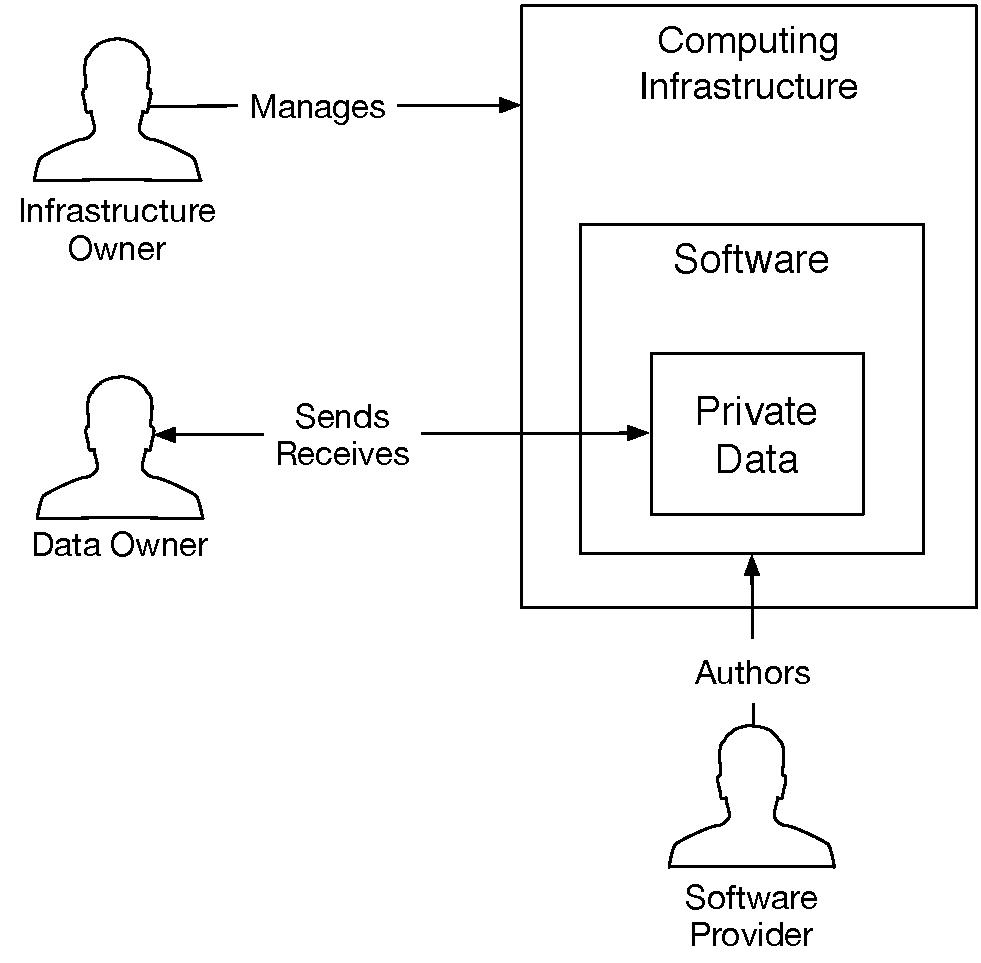
\includegraphics[width=75mm]{figures/computing_model.pdf}
  \caption{
    The computing model assumed by our system. The infrastructure owner,
    software provider and data owner mutually distrust each other. Our system
    aims to guarantee that the private data will not leak even if the software
    is malicious and cooperates with a malicious infrastructure, or with
    another malicious piece of software running on the infrastructure.
  }
  \label{fig:computing_model}
\end{figure}

\subsection{Motivation}
\label{sec:motivation}

The most popular instance of the above problem is cloud computing using public
clouds. For example, CheapoTax, a software provider, might provide tax return
preparation software as a service running on Amazon's public cloud. Users
upload their financial information, encrypted using TLS, to Amazon data
centers, where CheapoTax's computation uses the data to produce tax returns,
which are downloaded by the users in an encrypted form, using TLS. Currently,
the users must trust that neither Amazon nor CheapoTax will record their
private financial information. Users must also hope that neither Amazon's
infrastructure nor CheapoTax's software have bugs that would allow other rogue
actors to obtain the private financial data by running malicious software in
the same public Amazon cloud used by CheapoTax.

Another example of the problem we are aiming to solve is a multiplayer game of
any genre, such as League of Legends \cite{riot2009lol},
World of Warcraft \cite{blizzard2004wow}, StarCraft \cite{blizzard2010sc2}, and
Doom \cite{id2004doom}. The gameplay of many multiplayer games, such as the
ones listed above, rely on the fact that that players can only access a subset
of the game state that is dictated by the units they control. To compensate for
network latencies, many games entrust a player's game client with a superset
of the game state that the user should have access to. For example, in
StarCraft, the game client code running on the players' computers ``knows'' the
entire state, and is trusted to hide the information that the player should not
have access to \cite{hardy2009cheating}. The other games metioned above also
store information that the player shouldn't access in the game clients, leading
to opportunities for cheating \cite{youtube2013lolcheating}
\cite{youtube2008quake3cheating}.


\subsection{Threat Model}
\label{sec:threat}

Our threat model assumes that the infrastructure is shared by multiple ongoing
computations, potentially using software from different mutually distrusting
providers. The operating system and high-level software used to manage the
infrastructure may be malicious, and may cooperate with one or more malicious
pieces of software running on the infrastructure, including the software that
performs computations on the private data that must be protected, to accomplish
a \textbf{software attack}. The infrastructure owner may also mount a
\textbf{physical attack} by attaching a device to one of the computer's buses,
such as the DDR3 bus used for DRAM accesses, or the PCI express bus. We
consider physical attacks to be significantly more expensive to carry out than
software attacks, and we treat them separately where it makes sense to do so.

The threat model accurately represents a public cloud. Attackers can rent
resources and run malicious software, as well as run experiments to reveal and
exploit vulnerabilities in the infrastructure software. The programs that run
over the private data can also have vulnerabilities, which can be exploited by
attackers. An attacker can also motivate a datacenter maintenance employee to
attach a physical device to a server, but this attack is significantly harder
to mount than a purely software attack.

At the same time, a software attack that takes control of the kernel or
hypervisor can be used to reflash a computer's BIOS \cite{wojtczuk2010bios}. On
computers with Intel's Active Management Technology (AMT) \cite{intel2013amt},
the flash memory chip containing the BIOS code also contains the firmware
executed by the Manageability Engine (ME), a service processor that is embedded
in the Platform Controller Hub (PCH), shown in Figure \ref{fig:pch}. The ME can
access RAM via DMA, can communicate using the network, and can override the
CPU's boot vector, causing it to boot a malicious OS kernel or hypervisor
\cite{tereshkin2009amt}. Therefore, a software attack that escalates into
taking over the Intel ME can give the attacker powers that are traditionally
associated with hardware attacks, and this work treats it as a physical attack.

\begin{figure}[hbtp]
  \centering
  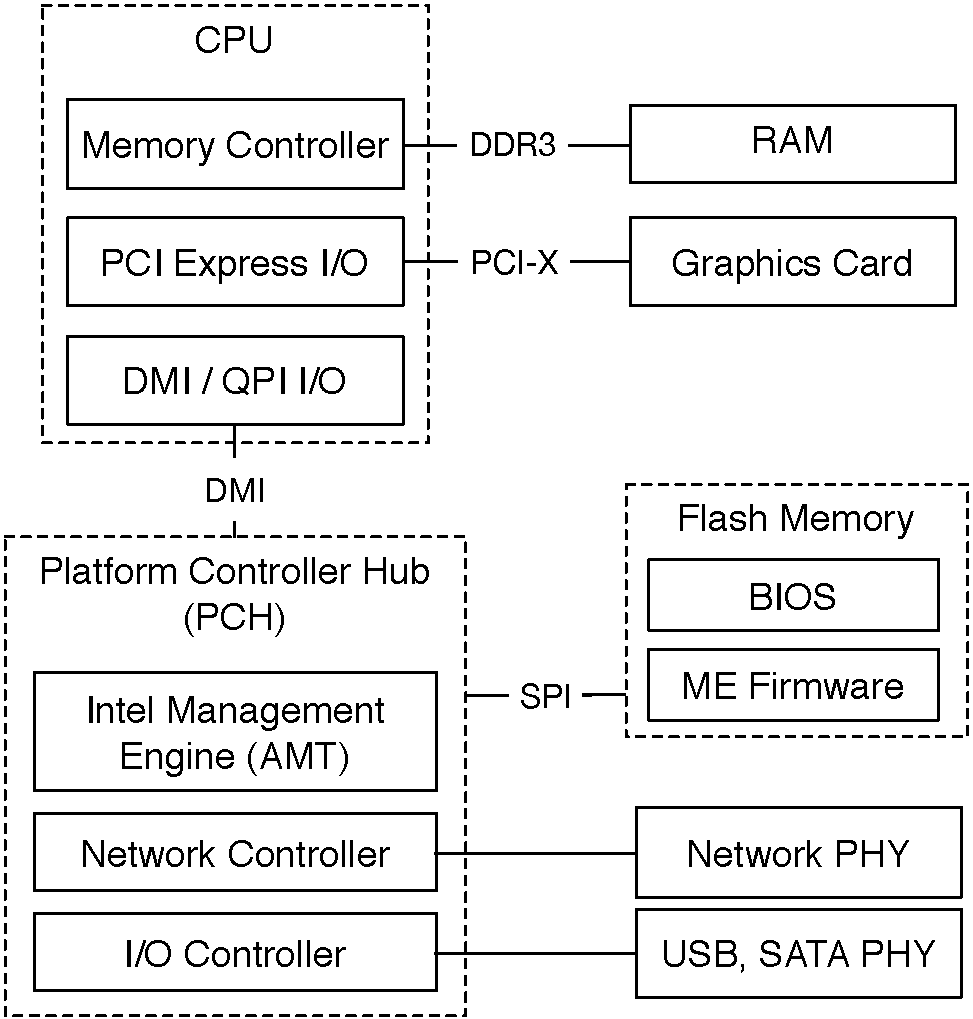
\includegraphics[width=65mm]{figures/pch.pdf}
  \caption{
    The Platform Controller Hub (PCH) contains a service processor, called the
    Intel Management Engine (ME). The processor has direct access to the
    network, can read and modify RAM via DMA transfers, and can override the
    CPU boot vector. The processor runs firmware stored in the same flash
    memory as the BIOS code.
  }
  \label{fig:pch}
\end{figure}

In the multiplayer game case, the private data is the full game state, and the
data owner is the same as the software supplier. The infrastructure is the
players' computers. Given that players have an incentive to cheat, it is
reasonable to assume that the infrastructure can behave maliciously. Our system
assumes that the players can exploit any vulnerability available in the game
software. Furthermore, players that desire an unfair advantage might install
software that is specifically designed for cheating. This software may be
running concurrently with the game software, and may include components that
run with OS privileges (e.g., Windows drivers or Linux / Darwin kernel
modules) or even SMM privileges (e.g., BIOS hacks). Last, players are willing
to attach hardware devices (known as \textit{mods} or \textit{modchips}) to
computers or game consoles to be able to cheat \cite{harris2007mod}, so
hardware attacks are even more relevant in the multiplayer game scenario.

Our threat model does not cover attacks that require intimate knowledge of the
processor's hardware internals. Most importantly, we do not protect against
malicious OS-level software that can abuse a CPU's in-field microcode update
mechanism to create a vulnerability in the processor's security features, or
against attackers that have knowledge of existing vulnerabilities in the CPU.
We also do not protect against attacks that analyze the computer's power
consumption.

Last, the threat model does not include denial of service attacks. Our system
requires the operating system that manages the infrastructure to enable certain
CPU features. We do not trust the operating system, so our system checks for
the features' presence and enablement. If the checks fail, the system refuses
to decrypt private data and to perform any computation. This can lead to a
denial of service attack. At the same time, an attack that compromises the
operating system can cause a denial of service simply by disabling the network
driver, and that cannot be worked around as long as the OS is untrusted.


\subsection{Challenges and Opportunities}

Our threat model is minimal given the constraint of being applicable to
commodity computers, in the sense that trusting the die that contains the CPU
is a prerequisite to being able to trust any computing performed by the CPU.

The challenge in providing trusting computing guarantees to software running on
commodity computers is that after 30 years of organic evolution, today's x86
CPUs expose many architectural features and privilege levels that interact in
complex ways. \S~\ref{sec:architecture_background} reviews these features and
mentions attacks that have compromised the software running at all privilege
levels, forcing us to conclude that we cannot rely on any software running on
the infrastructure.

The opportunity that our model brings is being able to take advantage of the
isolation mechanisms and the high level of integration in modern CPUs (see
Figure \ref{fig:cpu_die}). For example, the memory controller that used to be
relegated to a separate northbridge chip is now in the CPU, so it is part of
the TCB, and we can rely on it to enforce the memory isolation needed to
implement a protected execution environment, as explained in \S~\ref{sec:sgx}.
Today's CPUs also have on-die L2 and L3 cache memory, so we can rely on some
privacy and integrity for cache accesses, as detailed in \S~\ref{sec:caching}.

\begin{figure}[hbtp]
  \centering
  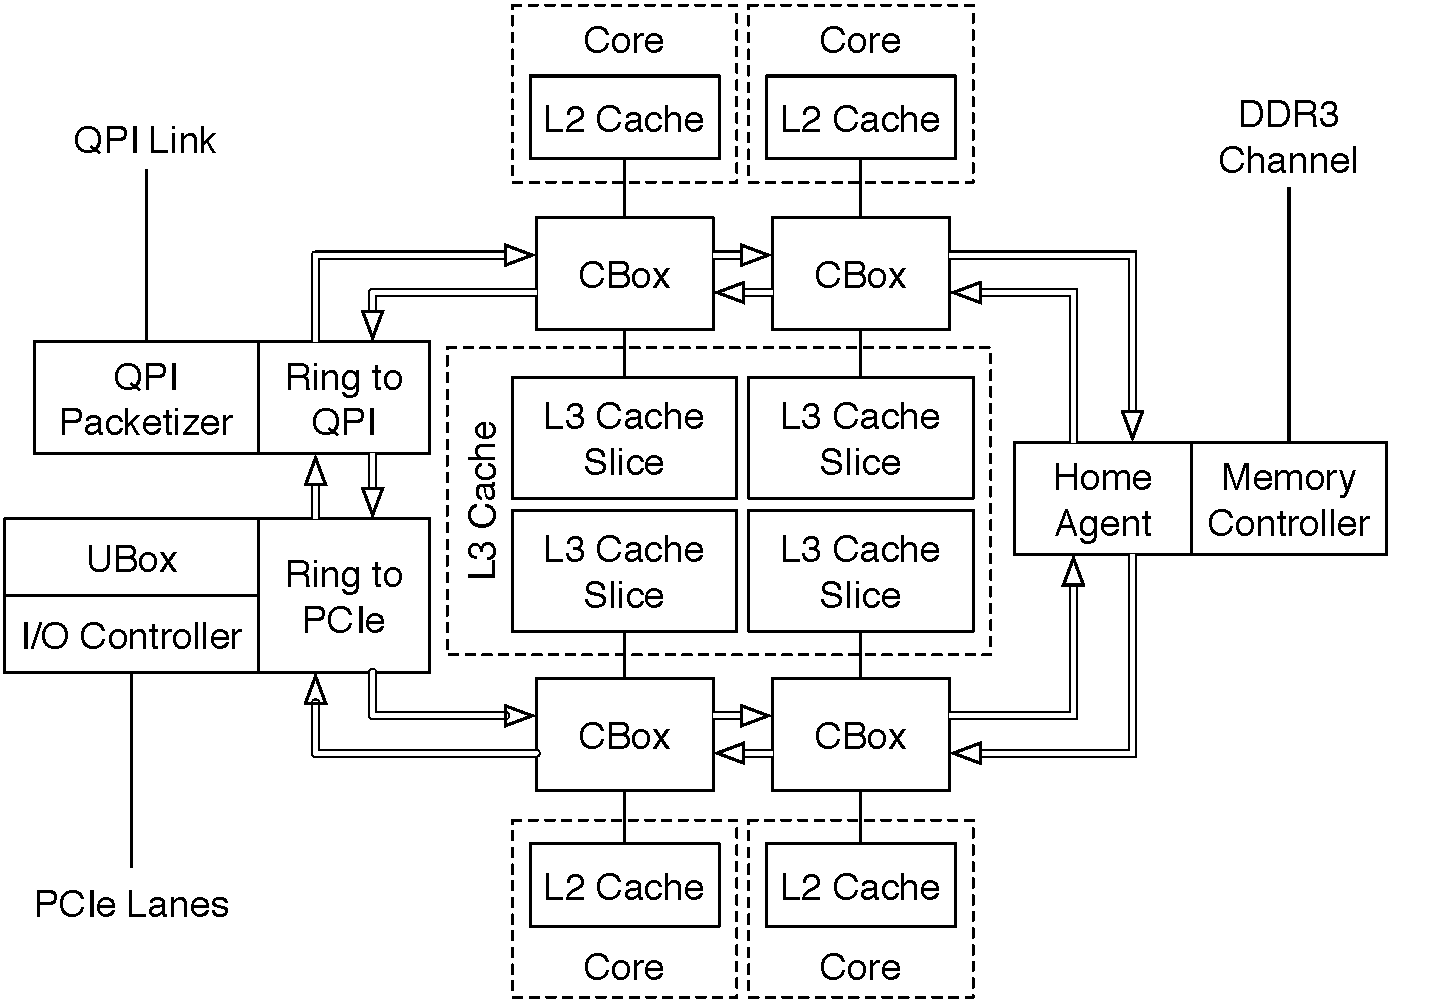
\includegraphics[width=85mm]{figures/cpu_die.pdf}
  \caption{
    A modern CPU die contains three levels of cache memory, as well as a
    memory controller. All these components are in our TCB.
  }
  \label{fig:cpu_die}
\end{figure}

Furthermore, we can take advantage of the CPU features for setting up isolated
execution environments. The currently deployed features are Intel's Trusted
Execution Technology (TXT) \cite{grawrock2009txt} and AMD's Secure Virtual
Machine (SVM) \cite{strongin2005trusted}, which is functionally similar to TXT.
Unfortunately, TXT requires a hypervisor and a system initialization (SINIT)
module in the TCB, and the attacks mentioned in \S \ref{sec:rings} suggest that
the resulting TCB would be very difficult to secure. Therefore, we focus our
attention on Intel's Software Guard Exections (SGX) \cite{mckeen2013innovative}
\cite{anati2013sgx}.


\subsection{Towards Secure Computation}
\label{sec:approach}

\S \ref{sec:sgx} provides an overview of SGX and its interactions with other
CPU features, and argues that SGX provides integrity guarantees in our threat
model, but does not prevent a malicious hypervisor or OS from taking advantage
of address translation (\S \ref{sec:paging}) and caching (\S \ref{sec:caching})
to learn about the memory access patterns of the software protected by SGX,
which can be used to gain knowledge about the private data used in the
computation. For example, cache timing attacks can be used to recover
encryption keys \cite{bonneau2006cache} \cite{brumley2005remote}
\cite{kocher1996timing}.

In \S \ref{sec:design}, we outline a method for hiding an application's memory
access patterns by taking advantage of the L2 cache layout (see \S
\ref{sec:caching}) to control when data is evicted from the cache. We can use
an oblivious RAM protocol \cite{stefanov2013path} to hide the cache eviction
patterns. Unfortunately, our scheme still leaks memory access patterns under
the currently documented SGX design, due to page faults (\S \ref{sec:paging})
and asynchronous enclave exits (AEX). \S \ref{sec:design} We explore the
problem of devising a minimal set of changes to SGX that make our scheme work.
At the same time, we explore a scheme that can protect memory accesses under
the current SGX design, and that is more practical than fully-homomorphic
encryption \cite{gentry2009fhe} \cite{naehrig2011can}.
